\chapter{Data Analysis and Results}

In this chapter, I will summarize the raw data and the corresponding results. The chapter ends with a discussion on the sources of error in this experiment.
%-------------------------
%        RAW DATA
%-------------------------

\section{Raw Data}



The raw data consisted of a total of 7 videos. All of the variables collected for each trial are laid out in \reftab{datacollection}, and the raw data is presented in \refTab{raw} in the \textbf{Appendix}. Barrier height, acceleration of the tray, Faraday threshold, and percentage of ``transmissions" were recorded for each of the 7 videos. The 7 videos contained: one trial of a single droplet for all three barrier heights, another trial of a single droplet for all three barrier heights, and a final trial of a single droplet for the $3.0~\mathrm{mm}$ barrier.\footnote{A similar methodology was attempted for Trial 3, but droplet coalescence prevented a complete trial from being recorded. Eventually it was decided to only examine the middle of the 3 barrier, since it exhibited the richest behavior.} By switching the barriers while the tray was still shaking we were able to use same droplet for each of the three barrier heights in a trial. There were between 12 to 24 separate collisions for each barrier. An example of a trial is presented in \refFig{trialex}.

\begin{table}[h]
\caption{This table illustrates data collected for all trials. For each barrier ($2.75~\mathrm{mm}$, $3.0~\mathrm{mm}$, or $3.25~\mathrm{mm}$), the forcing acceleration $\gamma$, the Faraday threshold acceleration $\gamma_\mathrm{F}$, and the percentage of ``transmissions" (\%T) were recorded. The oil volume $V$ was recorded at the beginning of each trial. From \textit{Tracker}, measurements of the droplet diameter $D_n$ in three randomly selected frames were made, along with the velocity of the droplet for every frame $v(t)$. Using $V$, the values of the depth of oil in the bath $H$ and over the barrier $h$ were calculated.}
\begin{center}
\begin{tabular}{ccccc}

\hline
Trial & Barrier & Recorded & From \textit{Tracker}  & Calculated \\
\hline
\multirow{3}{*}{1} & 2.75 & $\gamma$, $\gamma_\mathrm{F}$, \%T, $V$ & {3 x }$D_1$, $v(t)$ & $H$, $h$ \\
                   & 3.0 & $\gamma$, $\gamma_\mathrm{F}$, \%T & {3 x }$D_1$, $v(t)$ & $H$, $h$   \\
                   & 3.25 & $\gamma$, $\gamma_\mathrm{F}$, \%T & {3 x }$D_1$, $v(t)$ & $H$, $h$  \\
                   \hline
\multirow{3}{*}{2} & 2.75 & $\gamma$, $\gamma_\mathrm{F}$, \%T, $V$ & {3 x }$D_2$, $v(t)$ & $H$, $h$ \\
                   & 3.0 & $\gamma$, $\gamma_\mathrm{F}$, \%T & {3 x }$D_2$, $v(t)$ & $H$, $h$   \\
                   & 3.25 & $\gamma$, $\gamma_\mathrm{F}$, \%T & {3 x }$D_2$, $v(t)$ & $H$, $h$  \\
                   \hline
\multirow{1}{*}{3} & 3.0 & $\gamma$, $\gamma_\mathrm{F}$, \%T, $V$ & {9 x }$D_3$, $v(t)$ & $H$, $h$ \\   
\hline         
                     
\end{tabular}
\end{center} 
\label{datacollection} 
\end{table}

%\begin{figure}[h!]
%	\centering
%	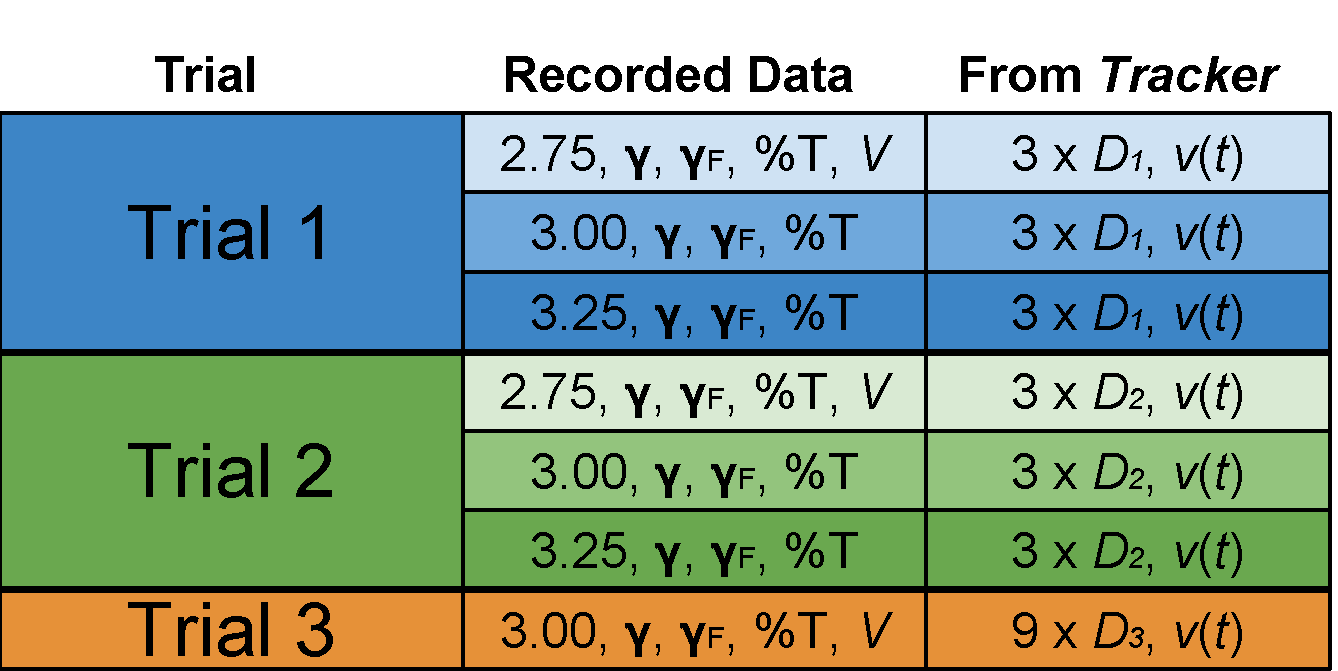
\includegraphics[scale=0.4]{datacollection.pdf}
%	\caption{For each barrier ($2.75~\mathrm{mm}$, $3.0~\mathrm{mm}$, or $3.25~\mathrm{mm}$), the forcing acceleration $\gamma$, the Faraday threshold acceleration $\gamma_\mathrm{F}$, and the percentage of ``transmissions" (\%T) were recorded. The oil volume $V$ was recorded at the beginning of each trial. From \textit{Tracker}, measurements of the droplet diameter $D_n$ in three randomly selected frames were made, along with the velocity of the droplet for every frame $v(t)$.}
%	\label{datacollection}
%\end{figure}

These movies were then processed with \textit{Tracker} \cite{tracker}. \textit{Tracker} decomposes a video into multiple frames for the purpose of tracking an object in a video. The Autotracker function marks the position of the object in every frame and records the time in between each frame ($\frac{1}{24}$ seconds). \textit{Tracker} uses this information to estimate the velocity of the droplet at every frame. We also want to know the size of each droplet, so we measure the diameter of the droplet using a function in \textit{Tracker}. The diameter is measured 3 times in each movie, yielding 9 total measurements per trial. These nine measurements were averaged to estimate the diameter of the droplet used in that trial. In trial 3, where only one barrier was used, 9 independent measurements were made, as detailed in \refSect{sect:error}.

\begin{figure}[h!]
	\centering
	\includegraphics[scale=0.58]{Trial2Paths.pdf}
	\caption{The the raw data from Trial 2. The red line in each image traces the path of the droplet for the duration of the trial. For each of the three barrier heights, the $h$ of the oil above the barrier is shown, along with the fraction of droplets $T$ that tunneled across the barrier. }
	\label{trialex}
\end{figure}

From the volume of the oil $V$ measured with a graduated cylinder, and measurements taken of the $178~\mathrm{mm}$ diameter tray, we can calculate the parameter $h$, which is defined as the height of the oil above the barrier. This was done by calculating the volume the ``space" inside the tray, which required knowing the dimensions of the tray accurately. Values for the various parameters in this experiment are shown in \reftab{explimits}. Error estimates are discussed in \refSect{sect:error}.%\footnote{The function making this calculation can be found in the Appendix.}
\renewcommand{\thefootnote}{\fnsymbol{footnote}}
	       \begin{table}[htdp] 
\caption[Basic Table 1]{Values of the various parameters in this experiment.} 
\begin{center} 
\begin{tabular}{c c} 
\toprule 
  Parameter &  Lower Limit\\
  \midrule
Viscosity $\nu$ (cSt) & $20.0$\tablefootnote{Value provided by the manufacturer.} \\ 
Frequency $f$ (Hz) & $80.0$ \\
Density $\rho$ (g/mL) & $0.95^{\dagger}$ \\
Memory $\gamma/\gamma_\mathrm{F}$ & $0.98 \pm 0.03 $ \\
Drop Diameter $D$ (mm) & $0.99$ to $1.07 \pm 0.04$ \\
Bath Depth $H$ (mm) & $4.26 \pm 0.35$ \\
Oil Depth Above Barrier $h$ (mm) & $0.99$ to $1.52 \pm 0.35$ \\ 
\bottomrule 
\end{tabular}
\end{center}
\label{explimits} 
\end{table}	

\renewcommand{\thefootnote}{\arabic{footnote}}
%-------------------------
%        ANALYSIS
%-------------------------
\section{Analysis}


    \subsection{Tunneling vs. Oil Depth}
The primary purpose of this investigation was to determine how the depth of the fluid layer above the barrier affects tunneling. The results are shown in \refFig{tbh}, indicating that droplets never crossed near $h=1.0~\mathrm{mm}$, whereas they always crossed at a value $h=1.5~\mathrm{mm}$. For the intermediate depth $h=1.25~\mathrm{mm}$, both transmissions and reflections were observed at a rate that changes for every trial. If we consider the droplet diameter, we see that the plot suggests that the transmission coefficient increases as the diameter of the droplet increases. 

The vertical error bars indicate standard error, and the horizontal error bars indicate uncertainty calculated using error propagation. 

\begin{figure}[h!]
	\centering
	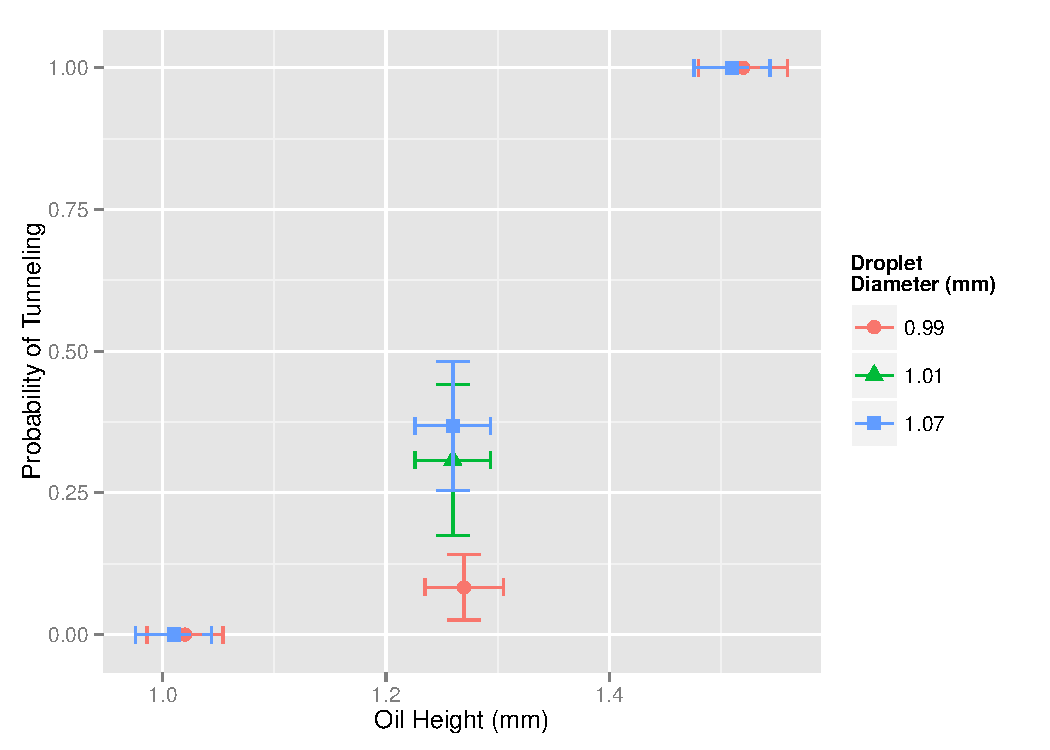
\includegraphics[scale=.9]{TunnelingProb.pdf}
	\caption{The proportion of collisions leading to transmission as a function of $h$. Each data series corresponds to a single trial for which the droplet diameter was kept constant.}
	\label{tbh}
\end{figure}


    \subsection{Tunneling by Droplet Velocity}
Not every droplet barrier collision was ideal. Many times, the droplets approached at an angle or at different velocities which means that it is a misleading to consider every collision as being the same. One way we can standardize collisions is by looking at the velocity perpendicular to the barrier at $5~\mathrm{mm}$ away from the center of the barrier, as shown in \refFig{tvd}.

\begin{figure}[h!]
	\centering
	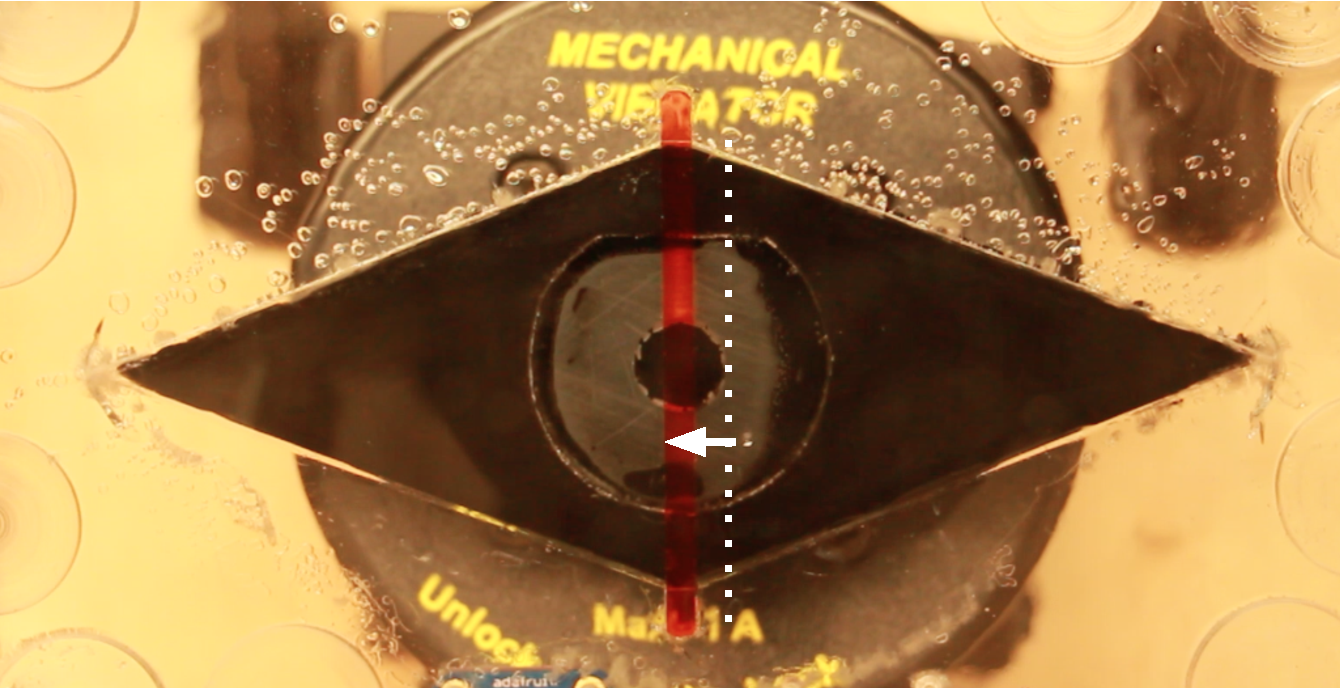
\includegraphics[scale=0.6]{TunnelingVDiagram.pdf}
	\caption{The image shows the point at which the measurement of the perpendicular component of velocity was made. This is $5~\mathrm{mm}$ from the middle of the barrier.}
	\label{tvd}
\end{figure}

We expect the perpendicular component of velocity to be important because it proved critical in the study of barrier width carried out by Eddi et al. \rf{tunneling}, and because it is intuitive: if the droplet moves faster, it has greater momentum and is more difficult to stop. \refFig{vel} shows every collision for the intermediate barrier height, and the result of each interaction. In trials 2 and 3, the droplets with the fastest perpendicular velocities were usually the ones that passed through the barrier, as expected. This did not seem to be the case for trial 1, for unknown reasons. 

\begin{figure}[h!]
	\centering
	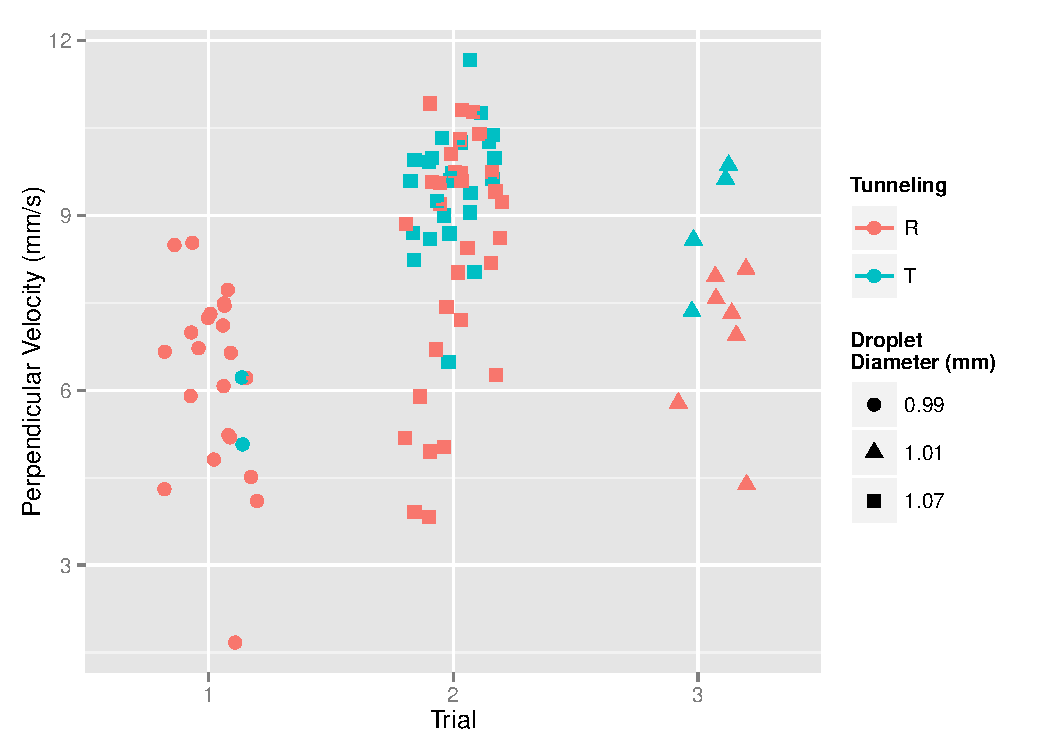
\includegraphics[scale=0.9]{Velocity2.pdf}
	\caption{The result of each collision for the intermediate oil depth. The color represents the outcome of the collision (either transmission (T) or reflection (R)), and the shape represents the diameter of the droplet. The horizontal spread within each trial was added to aid in visualization.}
	\label{vel}
\end{figure}

Next we try breaking up the collisions by velocity. The collisions from the $3.0~\mathrm{mm}$ barrier were grouped into bins of width $2~\mathrm{mm/s}$ and plotted by the fraction of all collisions that tunneled. The result, shown in \refFig{VP}, leaves a little to be desired. We see immediately the major limitation is the lack of trials, and perhaps, in consistency. Trial 3 is the only one that shows the expected trend for all bins: as velocity increases so does tunneling. Trial 2 starts off on the right track but a few reflections at high velocities skew the results. Finally, the results from trial 1 are completely out of line with the expected behavior.
\begin{figure}[h!]
	\centering
	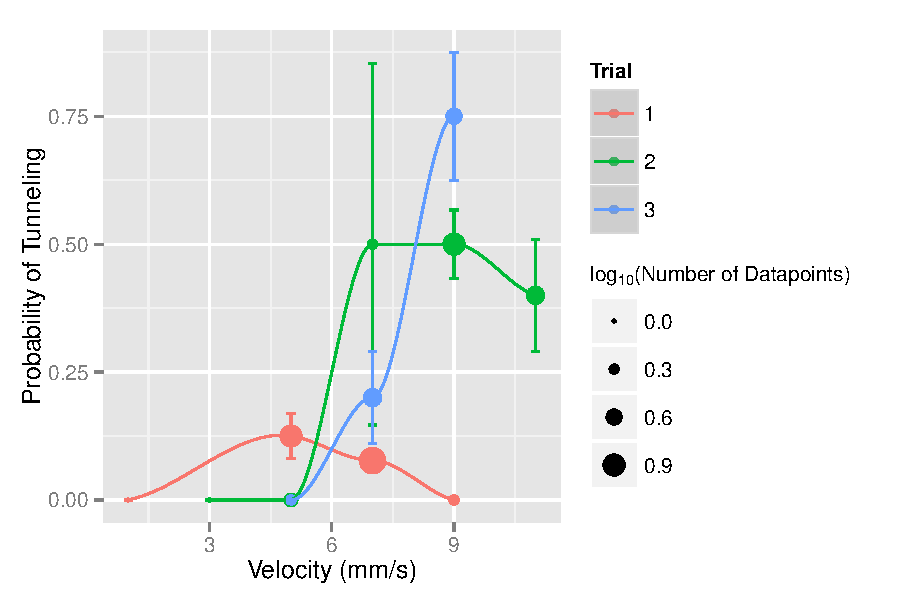
\includegraphics[scale=0.9]{VP.pdf}
	\caption{Collisions with similar perpendicular velocities were grouped into bins of width $2~\mathrm{mm/s}$ per bin. The overall fraction of transmissions was computed for each bin, and plotted. Colors distinguish between droplet diameters, and sizes indicate the number of data points in each bin. Error bars indicate the associated standard error. }
	\label{VP}
\end{figure}

Our data seem to indicate that tunneling probability increases as a function of velocity and of droplet diameter. Droplet diameter is really just a way of expressing the size of the droplet, but another way of doing that is by using the droplet's mass $m$. The momentum $p$ of an object of mass $m$ and velocity $v$ is defined as:
$$p = mv.$$
We can estimate the mass of the droplet by multiplying the volume of the droplet by its density $\rho$. Assuming a spherical droplet of diameter $D$, the volume is given by:
$$V_\mathrm{d} = \frac{4}{3}\pi \left(\frac{D}{2}\right)^3.$$
Thus, we can express the momentum of the droplet as
\begin{align}
p_\mathrm{d} &= \rho~V_\mathrm{d}~v \\
& = \rho~\frac{4}{3}\pi \left(\frac{D}{2}\right)^3 v
\end{align}
where the density $\rho$ of silicone oil has been provided by the manufacturer. Looking at just the perpendicular velocity component and grouping the droplets into bins (as we did in \refFig{VP}) and we get the plot shown in \refFig{fig:mom}. The plot shows incredibly similar slopes for portions of trials 2 and 3, suggesting the importance of momentum as a factor that increases tunneling probability. Even one of the momentum bins from the first trial falls on the curve, though the rest of the bins from that trial remain unexplained. 

\begin{figure}[h!]
	\centering
	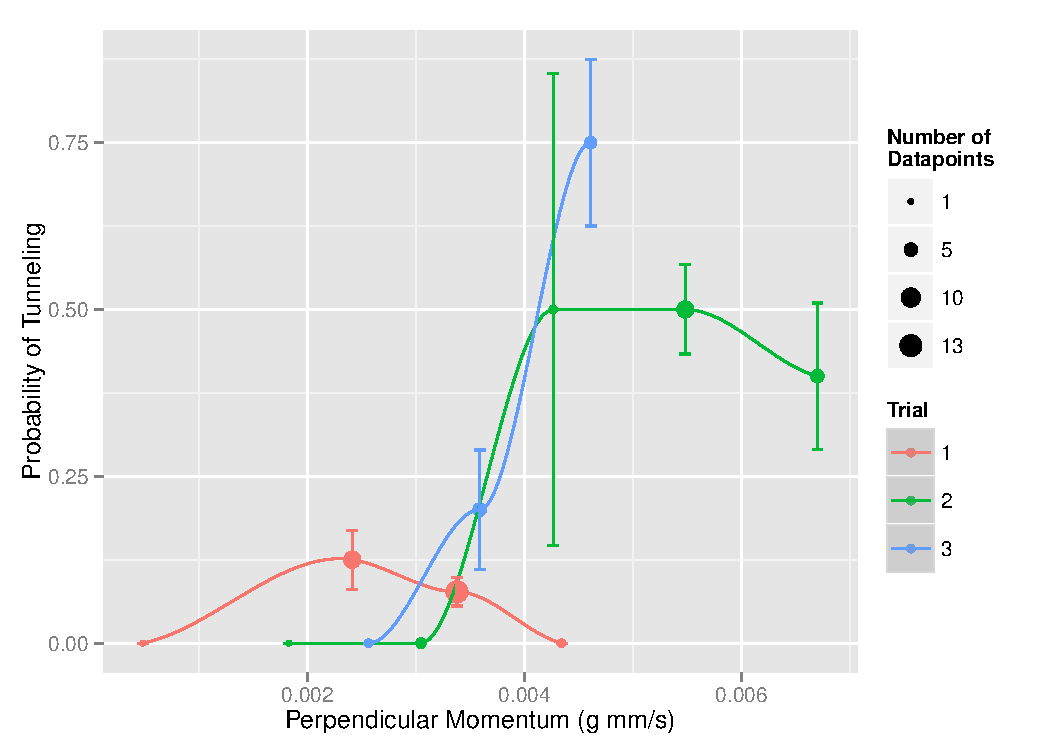
\includegraphics[scale=0.9]{Momentum.pdf}
	\caption{Collisions of similar perpendicular momentum were grouped into bins. The overall fraction of transmissions was computed for each bin, and plotted. Colors distinguish between trials, and sizes indicate the number of data points in each bin. Error bars indicate the associated standard error. }
	\label{fig:mom}
\end{figure}


%-------------------------
%       CONCLUSIONS
%-------------------------
%\section{Conclusions}


%-------------------------
%    SOURCES OF ERROR
%-------------------------
\section{Sources of Error}
\label{sect:error}

    With a system like the one studied here, which is sensitive to small variations in any parameter, it is crucial to keep track of the errors so that we can consider the limitations that these errors could have on our conclusions. Below, I discuss the nature of the experimental errors associated with my measurements.
       
    \subsection{Droplet Diameter}
    The droplet diameter measurements were made using the \textit{Tracker} program. Knowing the length (in mm) of another object in the frame, in this case the length of the rhombus cutout inside the tray, we can measure the length of anything else in the frame (in mm). This works by finding the length in mm associated with each pixel in the frame and finding the width in pixels of the droplet. Using this ratio $r_\mathrm{mtp}$, we can calculate the length of an object in mm:   
$$ 
\frac{\mathrm{length~of~rhombus~in~mm}}{\mathrm{length~of~rhombus~pixels}}= r_\mathrm{mtp} = \frac{\mathrm{diameter~of~droplet~in~mm}}{\mathrm{diameter~of~droplet~in~pixels}} 
$$ 
Since each pixel has a defined length, and because we cannot resolve anything within that pixel, our error is associated with that measurement is at least the width of half a pixel, usually around $\mathbf{0.04~\mathrm{\textbf{mm}}}$. There is also an error associated with the initial measurement of the rhombus in pixels, since it can be difficult to discern where exactly each point lies. This error was mitigated by making a new length measurement on \textit{Tracker} with every new barrier. 

Additionally, the droplet does not remain a perfect sphere as it bounces. At the bottom of its bounce, the droplet will be squished and appear (from the top view) wider than usual, where at the moment of lift it will be less wide (from the top) than usual. Since the camera recording our data shoots at 24 frames per second, it is impossible to know at what point in the bounce the droplet is, so it is impossible to know when to measure the diameter of the droplet. For this reason, we measured the diameter of the droplet in 3 random frames per at each of the 3 barrier heights, and with the total of 9 separate measurements per trial we averaged the results. Because the data for each barrier was filmed separately, this meant computing a new $r_\mathrm{mtp}$ value for each barrier. For the third trial in which only one barrier was used, the mm to pixel ratio $r_\mathrm{mtp}$ was re-calculated every 3 random diameter measurements, in order to mimic the procedure of the first two trials. In other words, 3 separate groups  of 3 measurements were made. Multiple measurements gave us an associated standard error, which combined with the error due to pixel limitations, gave us error bars. 

Our measurement procedure helped reduce the error associated with the changing size during a bounce. It also reduced the error associated with finding the exact value of $r_\mathrm{mtp}$ since, it was calculated 3 separate times each trial.

    \subsection{Droplet Velocity}
The droplet velocity was measured using \textit{Tracker}. The error in this measurement can be attributed to the Autotracker function, which automatically tracks the motion of the droplet using a built-in algorithm that searches a specific region of a frame for an known arrangement of pixels. Autotracking is mostly spot on, but if left alone for $1,000$ frames, the marker begins to deviate from the actual location of the droplet. The marker was adjusted whenever a deviation was noticed. The error can be estimated to no more than 10 pixels over $1000$ frames, corresponding to $\mathbf{\pm~0.01~\mathrm{\textbf{mm/s}}}$. However, because the measurement is being made at $5~\mathrm{mm}$ from the barrier, the uncertainty the velocity measurement becomes negligible.
    \subsection{Height of Oil}
The volume of oil was measured before each trial with a graduated cylinder with markings every half milliliter. With measurements on the order of $18.0~\mathrm{mL}$, there was an associated error of $\mathbf{\pm~0.10~\mathrm{\textbf{mL}}}$. Then, oil was lost between barrier adjustments since pliers were inserted in the oil to pull each barrier out, and a little bit of oil remained on the barrier and on the pliers each time. The volume of fluid lost after each barrier replacement was estimated to be about 3 droplets of diameter $3.0~\mathrm{mm}$. This corresponds to a loss of $\mathbf{0.014~\mathrm{\textbf{mL}}}$ of oil after every change in barrier. Finally, the volume of the oil was used to estimate the height of the oil above the barrier. The elements in the tray were manufactured for this experiment, and were then measured using digital calipers yielding an error of $\mathbf{\pm~0.03~\mathrm{\textbf{mm}}}$. 

For the height of the oil above the barrier, the above estimates provide us with an error on the order of about $\mathbf{\pm~0.35~\mathrm{\textbf{mm}}}$. The amount of fluid lost after each barrier replacement corresponds to a height decrease of $\mathbf{0.36~\mathrm{\textbf{mm}}}$ (for a barrier of the same size). This difference was offset by the added volume of the larger barrier, so that the bath depth $H$ remained relatively constant across the entire trial. 

It's impossible to account for factors such as the amount of oil left in the graduated cylinder, or the oil that may have seeped into microscopic fractures inside the tray. We assume these systematic errors to remain relatively constant over the duration of the experiment. This means that the pattern of our results should remain about the same, even if the exact numbers are slightly off. 

    \subsection{Consistency of Memory}
The shaker's acceleration decayed the longer it ran which lead to changes in droplet behavior. This could be seen by the acceleration measured by the accelerometer, which decreased even as the input signal remained constant. To counteract the changing acceleration, the amplitude of the driving signal was increased so that the system memory $\gamma/\gamma_\mathrm{F}$ remained constant (as measured by the accelerometer) throughout the length of the experiment. After replacing each barrier, the Faraday threshold $\gamma_\mathrm{F}$ was re-measured. As the amount of oil and the barrier height changed, the Faraday threshold also changed, so keeping the same input signal was not an option. Rather, in all experiments the \textit{memory} was kept constant, at $\gamma/\gamma_\mathrm{F} = \mathbf{0.98~\pm~0.03}$. Because at different memories we see different droplet behaviors, a constant memory meant we keep the droplet behavior as consistent as possible over the course of a trial \rf{Harris2013}. 

    \subsection{Imperfect Droplet Motion}
The intent of the tray design was to create droplet trajectories such that their collisions were perpendicular to the length of the barrier. However, in practice, this was not the case. Trajectories tended to deviate to one side and impacted the barriers at an angle. These trajectories tended to drift to the side of the tray with the accelerometer (shown in the top of \refFig{trialex}), possibly because the accelerometer added weight to one side causing the tray to vibrate unevenly. Often, in situations in which the droplet was reflected, the trajectory would cycle through a triangular orbit before diverging off in another path. This meant for a couple of collisions in a row, the droplet-barrier collision was not ideal since it was not completely perpendicular.

The perpendicular velocity measurements were a work-around since they provide a more descriptive picture of each interaction. Even with this crutch though, the angled trajectories are a symptom of an imperfect setup. Though great care was taken to ensure that the tray was flat, it was impossible to adjust the mostly vertical direction of vibration to be perfectly vertical. When the oscillations are not exactly vertical, the oil inside the tray does not shake evenly and it is not at a constant depth throughout the tray, which leads to imperfect droplet motion. Rather than moving in a straight line until encountering a barrier of some sort, the droplet will slowly curl away from certain areas within the tray. Additionally, the tray in our setup was attached at a single point by a rod connected to the shaker. This could have lead to bending of the acrylic at the edges, since the tray was so large. A mechanical shaker, as detailed in \rf{shaker}, would provide a much better base than the smaller shaker used in this experiment. It also has the added benefit of shaking the entire tray at once, rather than just a single point. While the error due to this component cannot be measured quantitatively, it should be considered when drawing conclusions.




